\documentclass{beamer}
\usepackage{amsmath,amssymb}
\usepackage{mathrsfs}  % for \mathscr
\usepackage{tabularx}
\usepackage{booktabs}
\usepackage{enumitem}   %列表
\setlist[enumerate]{itemsep=1pt,topsep=0pt,parsep=1pt }
\setlist[itemize]{itemsep=1pt,topsep=0pt,parsep=1pt, label=\textbullet}
% === collegeBeamer.sty options 可用选项 ===
%
% --- University/Institute Options 大学/机构 ---
% --- Language Options 语言 ---
% [en]     % English, pls compile with pdflLaTeX 英语,请使用 pdflLaTeX 编译
% [zh]     % Chinese, automatically loads xeCJK and Chinese fonts, pls compile with XeLaTeX 中文,自动加载 xeCJK 包和中文字体,请使用 XeLaTeX 编译
%
% --- Example Usage ---
\usepackage[zh]{collegeBeamer}
\usetikzlibrary{patterns}
\usetikzlibrary{calc} 

% user-defined commands
\newcommand{\dd}{\mathrm{d}}
\newcommand{\QUE}[1]{\noindent\boxed{\textbf{Question}} \textit{#1}\newline}
\newcommand{\ANS}{\noindent\boxed{\textbf{Solution}}\vspace{1mm}}
% \newcommand{\QUE}[1]{\noindent\boxed{\textbf{问 题}} \textit{#1}\newline}
% \newcommand{\ANS}{\noindent\boxed{\textbf{解 答}}\vspace{1mm}}

\newcommand{\COM}[1]{\texttt{#1}}
\newcommand{\QED}{\hfill\(\square\)}
\newcommand{\END}{\vspace{3mm}\hrule\vspace{3mm}}

% meta-data
\title{光学\ 习题课}
\subtitle{\textbf{第一次作业} Optics Lecture - $1^{\rm st}$ Homework}
\author{\textit{吴友鹏} \ \ \tiny (Youpeng Wu)}
\date{Sep 30, 2025}

% document body
\begin{document}
    
\maketitle

\begin{frame}{作业题目列表}

\begin{table}[htbp]
\centering
\renewcommand{\arraystretch}{1.2}
\begin{tabularx}{\textwidth}{@{}l|X@{}}
\toprule
章节 & 题目编号 \\
\midrule
第二章 几何光学基本原理 & 2.5, 2.8, 2.10, 2.16 \\
\midrule
第三章 光波衍射的标量波理论 & 
第四节 圆孔、圆屏的费涅尔衍射:3.3, 3.4 \\
\bottomrule
\end{tabularx}
\end{table}
\end{frame}

\section{第二章 几何光学基本原理\\ Chapter 2 Geometrical Optics Fundamentals}

% \themecolor{emptybg} 
\begin{frame}{Chapter 2}
\QUE{2.5 试用费马原理证明通过旋转双曲面一个焦点的光线经旋转双曲面反射后,其反射延长线经过另一个焦点}

\ANS 

由费马定理:光在两点间传播时,总是沿着光程为最小值的路径传播。我们构造这样一个证明: 对于从焦点 \(F_1\) 出发,经过旋转双曲面在点\(P\)反射后到达\(Q\)的光程, 在\(QP\)的延长线经过另一个焦点\(F_2\)时取得最小值。

对于双曲面上的点\(P\), 有关系
\[
|PF_2|-|PF_1|=2a \to |PF_1|=|PF_2|-2a
\]
而光程为
\[
L=|PF_1|+|PQ|=|PF_2|+|PQ| -2a
\]
当光程取最小时, \(L\) 取最小值, 则此时\(P\), \(Q\), \(F_2\) 三点共线, 即光线的反射延长线经过另一个焦点\(F_2\).

\QED

\end{frame}


\begin{frame}{Chapter 2}

\fbox{\begin{minipage}[c]{\textwidth}
    \setlength{\fboxsep}{0pt}%
    \setlength{\fboxrule}{0.5pt}%
    \centering
    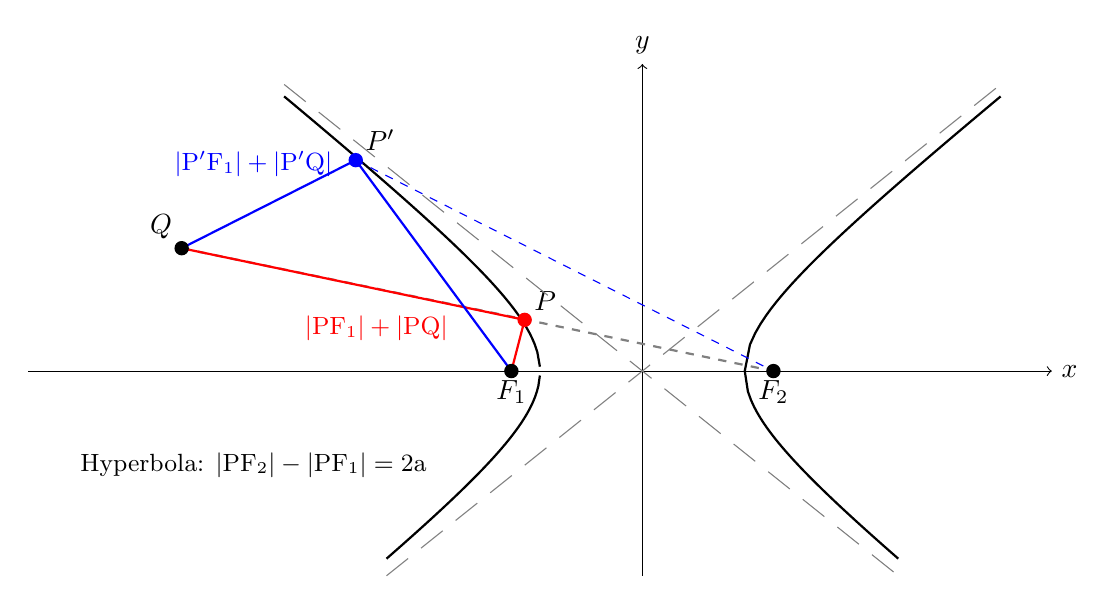
\begin{tikzpicture}[scale=1.3]
    % 坐标轴
    \draw[->] (-6,0) -- (4,0) node[right] {$x$};
    \draw[->] (0,-2) -- (0,3) node[above] {$y$};
    
    % 双曲线参数: a=1, b=0.8, c=1.28
    % 左支
    \draw[thick, black] plot[domain=-3.5:-1, samples=100] 
        (\x, {0.8*sqrt(\x*\x - 1)});
    \draw[thick, black] plot[domain=-2.5:-1, samples=100] 
        (\x, {-0.8*sqrt(\x*\x - 1)});
    % 右支
    \draw[thick, black] plot[domain=1:3.5, samples=50] 
        (\x, {0.8*sqrt(\x*\x - 1)});
    \draw[thick, black] plot[domain=1:2.5, samples=50] 
        (\x, {-0.8*sqrt(\x*\x - 1)});
    
    % 焦点
    \node[below] at (-1.28,0) {$F_1$};
    \node[below] at (1.28,0) {$F_2$};
    
    % Q点
    \coordinate (Q) at (-4.5, 1.2);
    \node[above left] at (Q) {$Q$};
    
    % P点(精确交点,已计算得 x ≈ -1.15, y ≈ 0.295)
    \coordinate (P) at (-1.15, 0.50);
    \node[above right] at (P) {$P$};
    
    % P'点(另一个左支点,x = -2.8, y = 0.8*sqrt(2.8^2-1) ≈ 2.06)
    \coordinate (Pprime) at (-2.8, 2.06);
    \node[above right] at (Pprime) {$P'$};
    
    % Q-F2连线 (蓝色虚线)
    \draw[gray, thick, dashed] (Q) -- (1.28,0);
    
    % 实际光线: F1 -> P (红色实线)
    \draw[red, thick] (-1.28,0) -- (P);
    % 实际光线: P -> Q (红色实线)
    \draw[red, thick] (P) -- (Q);
    
    % 假想光线: F1 -> P' (灰色虚线)
    \draw[blue, thick] (-1.28,0) -- (Pprime);
    % 假想光线: P' -> Q (灰色虚线)
    \draw[blue, thick] (Pprime) -- (Q);
    % 辅助线: P' -> F2 (灰色细虚线)
    \draw[blue, thin, dashed] (Pprime) -- (1.28,0);
    
    \fill[black] (-1.28,0) circle (2pt);
    \fill[black] (1.28,0) circle (2pt);
    \fill[black] (Q) circle (2pt);
    \fill[red] (P) circle (2pt);
    \fill[blue] (Pprime) circle (2pt);
%   % 顶点
%   \fill[black] (-1,0) circle (1pt);
%   \fill[black] (1,0) circle (1pt);
%   \node[below] at (-1,0) {$-a$};
%   \node[below] at (1,0) {$a$};
    
    % 光程标注
    \node[red, above] at (-2.6, 0.2) {\small $|\rm PF_1|+|\rm PQ|$};
    \node[blue, above] at (-3.8, 1.8) {\small $|\rm P'F_1|+|\rm P'Q|$};

    % 渐近线
    % 渐近线的斜率为 b/a = 0.8
    % y = 0.8x 和 y = -0.8x
    \draw[gray, thin, dash pattern=on 10pt off 6pt] (-2.5, {-0.8*2.5}) -- (3.5, {0.8*3.5});
    \draw[gray, thin, dash pattern=on 10pt off 6pt] (-3.5, {0.8*3.5}) -- (2.5, {-0.8*2.5});

    \node[black, below] at (-3.8, -0.7) {\small Hyperbola: $|\rm PF_2|-|\rm PF_1|=2a$};
\end{tikzpicture}
\end{minipage}}

\end{frame}

\begin{frame}{Chapter 2}
\QUE{2.8 光线以入射角\(i\)从折射率为\(n_w\)的水中入射到折射率为\(n\)厚度为\(h\)的玻璃中, 玻璃的折射率大于水的折射率. 计算光线在玻璃中的光程\(L\)}

\ANS

进入玻璃后, 光线的折射角为:
\[
n \sin r = n_w \sin i \to \sin r = \frac{n_w}{n} \sin i
\]
设光线在玻璃中的传播距离为\(d\), 则有:
\[
h = d \cos r \to d = \frac{h}{\cos r} = \frac{h}{\sqrt{1-\sin^2 r}} = \frac{h}{\sqrt{1-\left(\frac{n_w}{n}\sin i\right)^2}}
\]
光程为:
\[
L = n d = \frac{n h}{\sqrt{1-\left(\frac{n_w}{n}\sin i\right)^2}}= \frac{n^2 h}{\sqrt{n^2 - n_w^2 \sin^2 i}}
\]
\end{frame}

\begin{frame}{Chapter 2}

\QUE{2.10 光线经折射率为\(n\)的球形水珠折射. 求折射后光线偏向角的最大值}

\ANS

光线进入水珠后会发生两次折射, 设入射角为\(\alpha\), 折射角为\(\beta\). 则有:
\[
\sin \alpha = n \sin \beta \to \beta = \arcsin \frac{\sin \alpha}{n}
\]
光线偏向角\(\theta\)为:
\[
\theta = 2(\alpha - \beta) = 2\alpha - 2 \arcsin \frac{\sin \alpha}{n}
\]
对\(\alpha\)求导:
\[
\frac{d\theta}{d\alpha} = 2 - \frac{2 \cos \alpha}{n \sqrt{1-\left(\frac{\sin \alpha}{n}\right)^2}} = 0
\to 2 = \frac{2 \cos \alpha}{n \sqrt{1-\left(\frac{\sin \alpha}{n}\right)^2}}
\to n \sqrt{1-\left(\frac{\sin \alpha}{n}\right)^2} =  \cos \alpha
\]
\end{frame}
\begin{frame}{Chapter 2}
当\(\alpha=\pi/2\)时, \(\theta\) 取得最大值:
\[
\theta_{max} = \pi - 2 \arcsin \frac{1}{n}
\]
\begin{minipage}[c]{0.4\textwidth}
    \centering
    


% Pattern Info
 
\tikzset{
pattern size/.store in=\mcSize, 
pattern size = 5pt,
pattern thickness/.store in=\mcThickness, 
pattern thickness = 0.3pt,
pattern radius/.store in=\mcRadius, 
pattern radius = 1pt}
\makeatletter
\pgfutil@ifundefined{pgf@pattern@name@_6mh2pgkdc}{
\makeatletter
\pgfdeclarepatternformonly[\mcRadius,\mcThickness,\mcSize]{_6mh2pgkdc}
{\pgfpoint{-0.5*\mcSize}{-0.5*\mcSize}}
{\pgfpoint{0.5*\mcSize}{0.5*\mcSize}}
{\pgfpoint{\mcSize}{\mcSize}}
{
\pgfsetcolor{\tikz@pattern@color}
\pgfsetlinewidth{\mcThickness}
\pgfpathcircle\pgfpointorigin{\mcRadius}
\pgfusepath{stroke}
}}
\makeatother
\tikzset{every picture/.style={line width=0.75pt}} %set default line width to 0.75pt        

\begin{tikzpicture}[x=0.75pt,y=0.75pt,yscale=-1,xscale=1]
%uncomment if require: \path (0,300); %set diagram left start at 0, and has height of 300

%Shape: Circle [id:dp47523115765045854] 
\draw  [pattern=_6mh2pgkdc,pattern size=12pt,pattern thickness=0.75pt,pattern radius=0.75pt, pattern color={rgb, 255:red, 155; green, 155; blue, 155}] (66.67,148.33) .. controls (66.67,104.89) and (101.89,69.67) .. (145.33,69.67) .. controls (188.78,69.67) and (224,104.89) .. (224,148.33) .. controls (224,191.78) and (188.78,227) .. (145.33,227) .. controls (101.89,227) and (66.67,191.78) .. (66.67,148.33) -- cycle ;
%Straight Lines [id:da7610905084348585] 
\draw  [dash pattern={on 4.5pt off 4.5pt}]  (145.33,148.33) -- (240.26,58.18) ;
%Straight Lines [id:da26122017173896583] 
\draw    (202.67,93.88) -- (212.67,188.55) ;
\draw [shift={(206.99,134.75)}, rotate = 83.97] [fill={rgb, 255:red, 0; green, 0; blue, 0 }  ][line width=0.08]  [draw opacity=0] (8.93,-4.29) -- (0,0) -- (8.93,4.29) -- cycle    ;
%Straight Lines [id:da08455822982829975] 
\draw  [dash pattern={on 4.5pt off 4.5pt}]  (202.67,93.88) -- (107.34,79.22) ;
\draw [shift={(150.06,85.79)}, rotate = 8.75] [fill={rgb, 255:red, 0; green, 0; blue, 0 }  ][line width=0.08]  [draw opacity=0] (8.93,-4.29) -- (0,0) -- (8.93,4.29) -- cycle    ;
%Straight Lines [id:da5652093586635702] 
\draw  [dash pattern={on 4.5pt off 4.5pt}]  (145.33,148.33) -- (248.3,209.83) ;
%Shape: Arc [id:dp4615412617607718] 
\draw  [draw opacity=0] (204.48,107.76) .. controls (203.89,107.84) and (203.28,107.88) .. (202.67,107.88) .. controls (198.62,107.88) and (194.99,105.99) .. (192.55,103) -- (202.67,93.88) -- cycle ; \draw   (204.48,107.76) .. controls (203.89,107.84) and (203.28,107.88) .. (202.67,107.88) .. controls (198.62,107.88) and (194.99,105.99) .. (192.55,103) ;  
%Shape: Arc [id:dp06900445719233972] 
\draw  [draw opacity=0] (200.37,181.88) .. controls (200.65,181.35) and (200.97,180.84) .. (201.33,180.34) .. controls (203.7,177.06) and (207.37,175.23) .. (211.22,175.01) -- (212.67,188.55) -- cycle ; \draw   (200.37,181.88) .. controls (200.65,181.35) and (200.97,180.84) .. (201.33,180.34) .. controls (203.7,177.06) and (207.37,175.23) .. (211.22,175.01) ;  
%Straight Lines [id:da8096367973292018] 
\draw    (212.67,188.55) -- (168.67,257.22) ;
\draw [shift={(194.18,217.41)}, rotate = 122.65] [fill={rgb, 255:red, 0; green, 0; blue, 0 }  ][line width=0.08]  [draw opacity=0] (8.93,-4.29) -- (0,0) -- (8.93,4.29) -- cycle    ;
%Straight Lines [id:da777128522091038] 
\draw    (202.67,93.88) -- (140.67,37.22) ;
\draw [shift={(167.98,62.18)}, rotate = 42.43] [fill={rgb, 255:red, 0; green, 0; blue, 0 }  ][line width=0.08]  [draw opacity=0] (8.93,-4.29) -- (0,0) -- (8.93,4.29) -- cycle    ;
%Shape: Arc [id:dp8738118911332267] 
\draw  [draw opacity=0] (224.39,195.71) .. controls (222.92,198.4) and (220.56,200.56) .. (217.53,201.68) .. controls (213.73,203.09) and (209.67,202.57) .. (206.34,200.61) -- (212.67,188.55) -- cycle ; \draw   (224.39,195.71) .. controls (222.92,198.4) and (220.56,200.56) .. (217.53,201.68) .. controls (213.73,203.09) and (209.67,202.57) .. (206.34,200.61) ;  
%Shape: Arc [id:dp5289496782411189] 
\draw  [draw opacity=0] (193.1,104.09) .. controls (192.66,103.69) and (192.25,103.25) .. (191.86,102.78) .. controls (189.28,99.65) and (188.44,95.64) .. (189.2,91.85) -- (202.67,93.88) -- cycle ; \draw   (193.1,104.09) .. controls (192.66,103.69) and (192.25,103.25) .. (191.86,102.78) .. controls (189.28,99.65) and (188.44,95.64) .. (189.2,91.85) ;  
%Shape: Arc [id:dp34734335147134476] 
\draw  [draw opacity=0] (193.16,83.98) .. controls (195.26,81.76) and (198.09,80.27) .. (201.31,79.95) .. controls (205.34,79.56) and (209.13,81.09) .. (211.86,83.83) -- (202.67,93.88) -- cycle ; \draw   (193.16,83.98) .. controls (195.26,81.76) and (198.09,80.27) .. (201.31,79.95) .. controls (205.34,79.56) and (209.13,81.09) .. (211.86,83.83) ;  

% Text Node
\draw (212.67,203.73) node [anchor=north west][inner sep=0.75pt]    {$\alpha $};
% Text Node
\draw (192,159.07) node [anchor=north west][inner sep=0.75pt]    {$\beta $};
% Text Node
\draw (190,109.73) node [anchor=north west][inner sep=0.75pt]    {$\beta $};
% Text Node
\draw (200,60.4) node [anchor=north west][inner sep=0.75pt]    {$\alpha $};
% Text Node
\draw (168.67,95.07) node [anchor=north west][inner sep=0.75pt]    {$\beta $};
% Text Node
\draw (228.67,174.4) node [anchor=north west][inner sep=0.75pt]    {$P_{1}$};
% Text Node
\draw (217.33,87.73) node [anchor=north west][inner sep=0.75pt]    {$P_{2}$};


\end{tikzpicture}

\end{minipage}
\begin{minipage}[c]{0.55\textwidth}
\textbf{球内多次反射}\newline
\COM{
如图所示, 在入射光线-球心平面上, 光线入射角为\(\alpha\), 折射角为\(\beta\). 当入射光线掠射入射时(沿切线方向), 入射角\(\alpha = \frac{\pi}{2}\), 此时折射角达到其最大值\(\beta_{max}=\arcsin \frac{1}{n}\), 即全反射角. 由于球的性质, 光线在球内的入射角也为\(\beta < \beta_{max}\).  所以对于一个理想的球形, 不会发生全反射, 此时光线射出. 从对称性的角度考虑会更加容易. \newline \pause
但是如果不在几何光学的条件下, 在小于全反射角的入射角下, 还是有部分光线会发生反射, 这时就会有多次反射的情况发生.
}
\end{minipage}
\end{frame}

\begin{frame}{Chapter 2}
    
\QUE{2.16 一个透明圆柱由厚度均匀的多层介质构成,各层介质均为圆筒状。已知由内向外各层介质的折射率和内半径分别为 \(n_l\) 和 \(r_l\),其中 \(l=1,2,\ldots,m\),光线在透明圆柱的截面内。求光线在各界面上的折射角 \(i_l\) 之间的关系。}

\ANS

光线在各层介质中的传播满足光线微分方程:
\[
\frac{d^2 \vec{r}}{d\tau^2}=n\nabla n
\]
由于这是一个柱对称的系统, 所以满足角动量守恒, 定义质量为1的粒子在各层介质中的角动量为:
\[
n_lr_l \sin i_l = \text{Const.} \quad (l=1,2,\ldots,m)
\]
所以此时:
\[
n_l r_l \sin i_l = n_k r_k \sin i_k = \text{Const.} \quad (l,k=1,2,\ldots,m)
\]
\end{frame}

\section{第三章 光波衍射的标量波理论\\ Chapter 3 Scalar Theory of Optical Diffraction}

\begin{frame}{Chapter 3}
    
    \QUE{3.3 一列光强为 \(I_0\),波长为 \(589.3\,\mathrm{nm}\) 的平面单色光波垂直入射到衍射屏上,衍射屏的透光部分为一个内直径等于 \(0.5\,\mathrm{mm}\),外直径等于 \(1.0\,\mathrm{mm}\) 的圆环。求距衍射屏 \(50\,\mathrm{cm}\) 处光轴上的光强。}
    
    \ANS 
    
    \begin{minipage}[c]{0.68\textwidth}
    分别计算圆孔中心-圆环内缘、圆环中心-圆环外缘的相位差:
        \begin{itemize}
            \item 圆孔中心-圆环内缘: \(\displaystyle \delta_1 = \frac{2\pi}{\lambda}\frac{d^2_1}{8b}=\frac{\pi d_1^2}{4\lambda b}\)
            \item 圆环中心-圆环外缘: \(\displaystyle \delta_2 = \frac{2\pi}{\lambda}\frac{d^2_2}{8b}=\frac{\pi d_2^2}{4\lambda b}\)
        \end{itemize}
    其中\(d_1=0.5\,\mathrm{mm}\), \(d_2=1.0\,\mathrm{mm}\), \(b=50\,\mathrm{cm}\), \(\lambda=589.3\,\mathrm{nm}\). 用矢量图得到待测广场的振幅:
    \[
    A=2A_0 \sin \left(\frac{\delta_2-\delta_1}{2} \right)
    \]
    \end{minipage}
    \begin{minipage}[c]{0.3\textwidth}
        \centering
        

\tikzset{every picture/.style={line width=0.75pt}} %set default line width to 0.75pt        

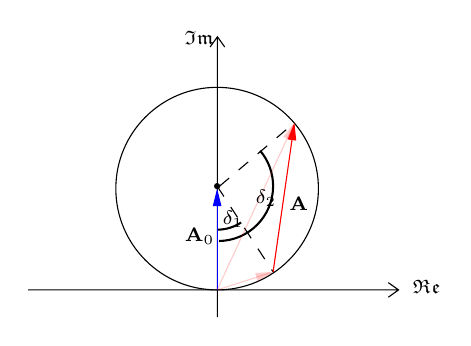
\begin{tikzpicture}[x=0.75pt,y=0.75pt,yscale=-0.7,xscale=0.7]
%uncomment if require: \path (0,300); %set diagram left start at 0, and has height of 300

%Shape: Axis 2D [id:dp7170454923860522] 
\draw  (89.19,230.52) -- (344.07,230.52)(219.41,56.28) -- (219.41,249.28) (337.07,225.52) -- (344.07,230.52) -- (337.07,235.52) (214.41,63.28) -- (219.41,56.28) -- (224.41,63.28)  ;
%Shape: Circle [id:dp8149789387083423] 
\draw   (149.48,160.8) .. controls (149.48,122.29) and (180.69,91.08) .. (219.2,91.08) .. controls (257.7,91.08) and (288.92,122.29) .. (288.92,160.8) .. controls (288.92,199.3) and (257.7,230.52) .. (219.2,230.52) .. controls (180.69,230.52) and (149.48,199.3) .. (149.48,160.8) -- cycle ;
%Shape: Circle [id:dp5023753623456884] 
\draw  [fill={rgb, 255:red, 0; green, 0; blue, 0 }  ,fill opacity=1 ] (217.47,159.06) .. controls (217.47,158.11) and (218.24,157.33) .. (219.2,157.33) .. controls (220.16,157.33) and (220.93,158.11) .. (220.93,159.06) .. controls (220.93,160.02) and (220.16,160.8) .. (219.2,160.8) .. controls (218.24,160.8) and (217.47,160.02) .. (217.47,159.06) -- cycle ;
%Straight Lines [id:da11025870442083607] 
\draw [color={rgb, 255:red, 0; green, 0; blue, 255 }  ,draw opacity=1 ]   (219.2,230.52) -- (219.2,162.8) ;
\draw [shift={(219.2,160.8)}, rotate = 90] [fill={rgb, 255:red, 0; green, 0; blue, 255 }  ,fill opacity=1 ][line width=0.08]  [draw opacity=0] (12,-3) -- (0,0) -- (12,3) -- cycle    ;
%Shape: Arc [id:dp502450717395721] 
\draw  [draw opacity=0][line width=0.75]  (235.73,184.1) .. controls (231.11,187.15) and (225.61,188.97) .. (219.69,189.06) -- (219.2,159.06) -- cycle ; \draw  [line width=0.75]  (235.73,184.1) .. controls (231.11,187.15) and (225.61,188.97) .. (219.69,189.06) ;  
%Shape: Arc [id:dp13047835740884117] 
\draw  [draw opacity=0][line width=0.75]  (248.84,134.71) .. controls (254.39,141.29) and (257.73,149.79) .. (257.73,159.06) .. controls (257.73,179.74) and (241.14,196.53) .. (220.55,196.86) -- (219.93,159.06) -- cycle ; \draw  [line width=0.75]  (248.84,134.71) .. controls (254.39,141.29) and (257.73,149.79) .. (257.73,159.06) .. controls (257.73,179.74) and (241.14,196.53) .. (220.55,196.86) ;  
%Straight Lines [id:da7593033774078591] 
\draw  [dash pattern={on 4.5pt off 4.5pt}]  (219.2,159.06) -- (257.73,218.13) ;
%Straight Lines [id:da8985109392556403] 
\draw  [dash pattern={on 4.5pt off 4.5pt}]  (220.93,159.06) -- (272.4,115.47) ;
%Straight Lines [id:da4308818839283928] 
\draw [color={rgb, 255:red, 255; green, 0; blue, 0 }  ,draw opacity=0.2 ]   (219.2,230.52) -- (271.56,117.28) ;
\draw [shift={(272.4,115.47)}, rotate = 114.82] [fill={rgb, 255:red, 255; green, 0; blue, 0 }  ,fill opacity=0.2 ][line width=0.08]  [draw opacity=0] (12,-3) -- (0,0) -- (12,3) -- cycle    ;
%Straight Lines [id:da598324613868965] 
\draw [color={rgb, 255:red, 255; green, 0; blue, 0 }  ,draw opacity=0.2 ]   (219.2,230.52) -- (255.83,218.75) ;
\draw [shift={(257.73,218.13)}, rotate = 162.19] [fill={rgb, 255:red, 255; green, 0; blue, 0 }  ,fill opacity=0.2 ][line width=0.08]  [draw opacity=0] (12,-3) -- (0,0) -- (12,3) -- cycle    ;
%Straight Lines [id:da7233738461447479] 
\draw [color={rgb, 255:red, 255; green, 0; blue, 0 }  ,draw opacity=1 ]   (257.73,218.13) -- (272.12,117.45) ;
\draw [shift={(272.4,115.47)}, rotate = 98.13] [fill={rgb, 255:red, 255; green, 0; blue, 0 }  ,fill opacity=1 ][line width=0.08]  [draw opacity=0] (12,-3) -- (0,0) -- (12,3) -- cycle    ;

% Text Node
\draw (352,221.73) node [anchor=north west][inner sep=0.75pt]  [font=\scriptsize]  {$\mathfrak{Re}$};
% Text Node
\draw (194.67,50.4) node [anchor=north west][inner sep=0.75pt]  [font=\scriptsize]  {$\mathfrak{Im}$};
% Text Node
\draw (195.2,186.07) node [anchor=north west][inner sep=0.75pt]  [font=\scriptsize]  {$\mathbf{A}_{0}$};
% Text Node
\draw (267.2,164.73) node [anchor=north west][inner sep=0.75pt]  [font=\scriptsize]  {$\mathbf{A}$};
% Text Node
\draw (243.87,160.07) node [anchor=north west][inner sep=0.75pt]  [font=\scriptsize]  {$\delta _{2}$};
% Text Node
\draw (221.2,174.73) node [anchor=north west][inner sep=0.75pt]  [font=\scriptsize]  {$\delta _{1}$};


\end{tikzpicture}

    \end{minipage}
\end{frame}

\begin{frame}{Chapter 3}
则观测点的光强为:
\[
I = |A|^2 = 4 I_0 \sin^2 \left(\frac{\delta_2-\delta_1}{2} \right) =4I_0 \sin^2 \left[\frac{\pi (d_2^2 - d_1^2)}{8\lambda b} \right]
\]
带入值可以得到:
\[
I=4I_0 \sin^2\left[\frac{\pi(d^2_2 - d^2_1)}{8\lambda b}\right] \approx 2.8 I_0
\]
\[
\text{Where} \quad d_1=0.5\,\mathrm{mm}, \quad d_2=1.0\,\mathrm{mm}, \quad b=50\,\mathrm{cm}, \quad \lambda=589.3\,\mathrm{nm}
\]
\end{frame}


\begin{frame}{Chapter 3}

\noindent\boxed{\textbf{Solution 2}}\vspace{1mm}

我们可以使用积分进行计算, \(P\)为光轴屏上点, 

\begin{align*}
    \tilde{U}(P) &=\frac{-i}{\lambda }\iint_{\Sigma} \tilde{U}_0 \frac{\exp(ik r)}{z} \dd S \\
    &=\frac{-i}{\lambda z}\int_{r_1}^{r_2} \tilde{U}_0 \exp(ik \sqrt{z^2 + \rho^2}) 2\pi \rho \dd\rho \\
    &=\frac{-i}{\lambda z} 2\pi \left. e^{i k \sqrt{z^2 + \rho^2}} (\frac{1}{k^2}-\frac{i\sqrt{z^2-\rho^2}}{k})\right|_{r_1}^{r_2}  
\end{align*}
带入数值波长\(\lambda=589.3\,\mathrm{nm}\), 光屏距离\(z=50\,\mathrm{cm}\), 内外径\(r_1=0.25\,\mathrm{mm}\), \(r_2=0.5\,\mathrm{mm}\), 光强\(I_0\)与\(\tilde{U}_0\)的关系为\(I_0 =|\tilde{U}_0|^2\), 则有:
\[
|\tilde{U}(P)| ^2 \approx 2.80705 I_0
\]

\end{frame}
\begin{frame}{Chapter 3}

\fbox{
\begin{minipage}[c]{\textwidth}
    \begin{figure}
        \centering
        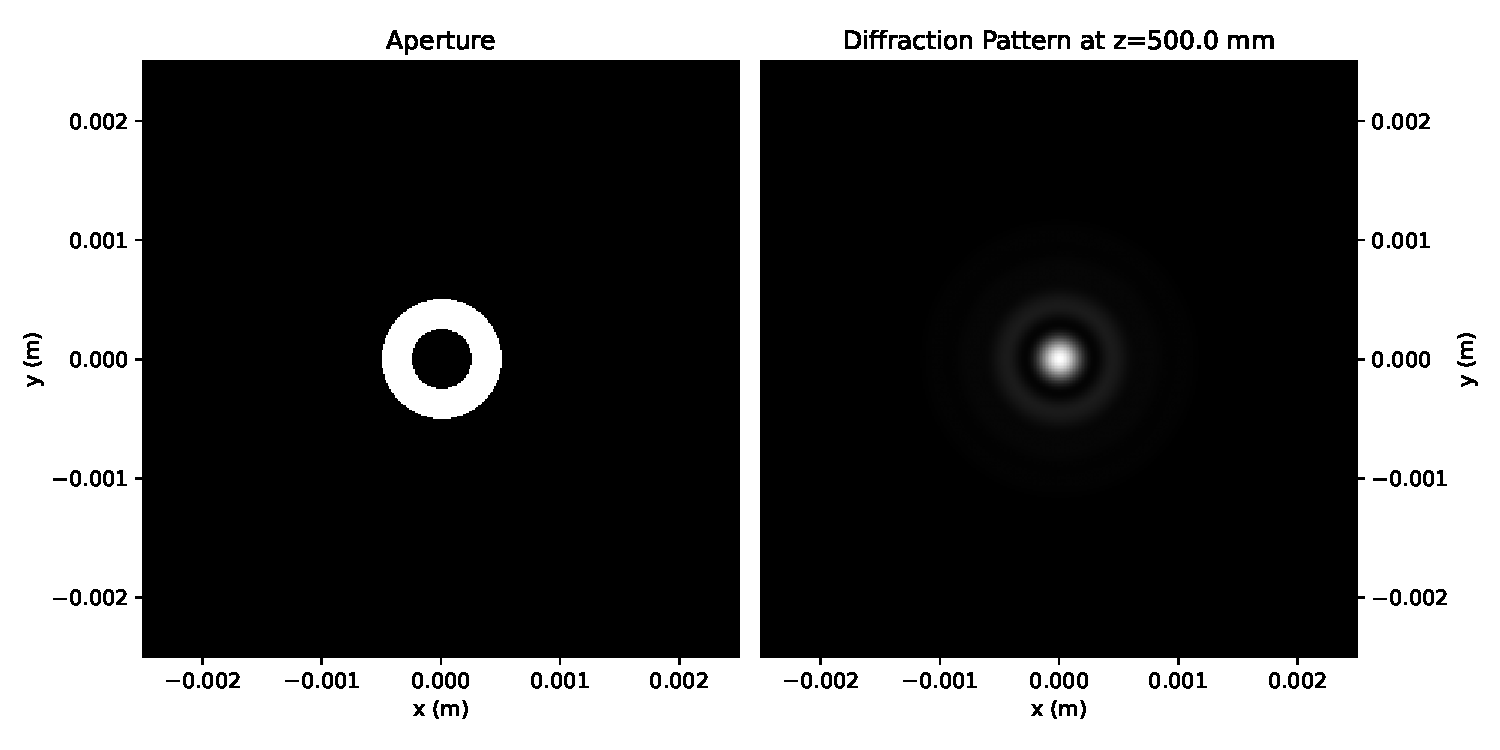
\includegraphics[width=0.8\textwidth]{figure/q3_3_diffraction_pattern.pdf}
    \end{figure}
    \[
    \tilde{U}(P) =\frac{-i}{\lambda }\iint_{\Sigma_0} \tilde{U}_0(\mathbf{r_0})\left[\frac{1}{2}(\cos \theta +\cos \theta_0)\right] \frac{\exp(ik|\mathbf{r}-\mathbf{r_0}|)}{|\mathbf{r}-\mathbf{r_0}|} \dd s_0
    \]
\end{minipage}
}

\end{frame}


\begin{frame}{Chapter 3}
    
    \QUE{3.4 用波长为 \(632.8\,\mathrm{nm}\) 的平面单色光波垂直照射衍射屏,衍射屏的透光部分为一个圆孔。已知在衍射屏后方距衍射屏 \(2.0\,\mathrm{m}\)、\(1.0\,\mathrm{m}\)、\(0.67\,\mathrm{m}\)、\(0.50\,\mathrm{m}\)、\(0.40\,\mathrm{m}\) 等处光轴上的光强为 0。求圆孔的直径。}

    \ANS 

\end{frame}
\QApage
        
\end{document}
